\section{Alpha Wave Analysis}\label{sec:alpha_test}
As mentioned in chapter \ref{ch:motivation} brain signals can be classified into four groups according to the dominant frequency \cite{EEGsignalprocessing}. 
It is known that when a person closes the eyes, when relaxing, the amount of alpha frequency raises and become the dominant frequency. 
The provided EEG measurements consist of measurements from a test subject with both open and closed eyes.
Hence, it would be interesting to investigate this relation between the alpha frequency for open and closed eyes. 
The interesting part is then to compare the relation achieve from the provided EEG measurements and the sources signals estimated by the main algorithm.

With a test of this kind, it is possible to evaluate the recovered source signals from a different perspective. 
Here the objective is first of all to see the behavior with respect to the frequency, expected by the theory. 
Next it is interesting to investigate the aspect of analysis performed on EEG level versus analysis performed on source level, as discussed in chapter \ref{ch:motivation}.              

\subsection{Test Setup}
For this comparison the data sets of test subject 1, \texttt{S1\_OClean} and \texttt{S1\_CClean}, EEG measurements of open and closed eyes respectively, will be used. 
It is expected that the power within the alpha frequency band is highest for the closed eyes data set, \texttt{S1\_CClean}.
To compare the amount of alpha frequency in the two data sets, a bandpass filter is used to isolate the alpha frequencies. 
To perform the filtering a bandpass Butterworth filter of order 5 with cut-off frequencies $8$ Hz and $13$ Hz will be applied. 
The filtering is performed in the time domain to both the EEG signals and the source signals recovered from the main algorithm.
The filtering process is illustrated in figure \ref{fig:dft_1}.
In the illustrated example only one source signal is investigated in both time and frequency domain, where the fast Fourier transformation (FFT) is applied \cite[Chapter 9]{FFT}. 
The source signal of interest was recovered from the closed eyes data set \texttt{S1\_CClean} from time segment $15$. 
The system specification used to recover the source signal was $M = 27$ and $k = 14$.
\begin{figure}[H]
\centering
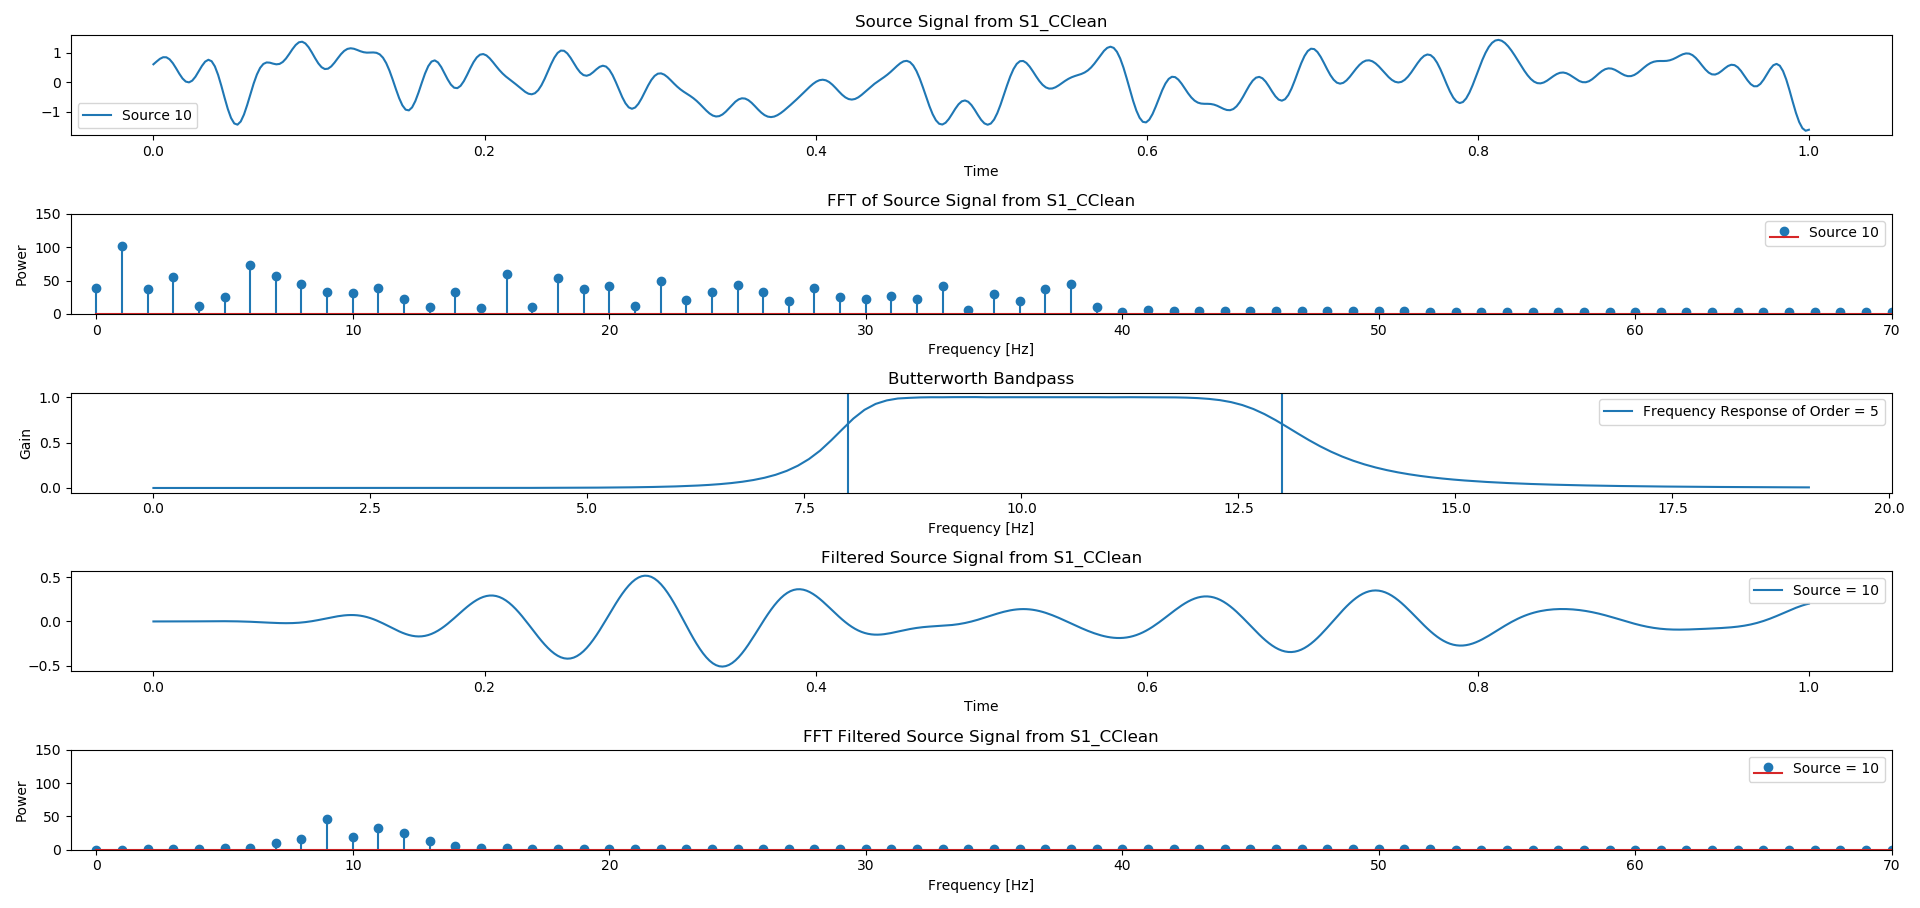
\includegraphics[scale=0.28]{figures/ch_7/DFT_plot_X_timeseg15_source10.png}
\caption{Time domain and frequency plot of a recovered source signal, filtered and non-filtered, from the time segment 15.}
\label{fig:dft_1}
\end{figure}
\noindent
The first plot in figure \ref{fig:dft_1} is the recovered source signal in the time domain. 
The next plot is the same source signal but transformed to the frequency domain by the FFT. 
The plot has been scaled to only show the frequencies from 0-70 Hz and the power from 0 to 150. 
The third plot illustrates the frequency response of the bandpass Butterworth filter with order 5. 
The vertical blue lines illustrate the cut-off frequencies at 8 Hz and 13 Hz.
Plot number four is the recovered source signal filtered by the bandpass Butterworth filter, plotted in the time domain. 
The last plot is the filtered source signal plotted in the frequency domain. 
This verifies that the signal of interest has been filtered according to the alpha band. 
From the filtered source signal in the time domain, the signal resemble the alpha wave as seen in figure \ref{fig:EEG_example}.

The filtering process is applied to 100 time segments of both the closed eyes and open eyes for respectively the EEG measurements and the recovered source signals. 
Note that for each time segment all present source signals or sensor measurements have been summed such that only one signal resembles each time segment.
Then for each time segment the relation between closed and open eyes is computed, with respect to power within the alpha band. 
The relation is defined as 
\begin{align*}
\text{Relation} = \frac{C}{O}, 
\end{align*}
where $C$ is the average power from closed eyes, and $O$ is the average power from the open eyes segment. 
This is done for both the EEG measurements and the recovered source signals. 
By this it is possible to compare the relation found on source level and the relation seen on EEG level.  

\subsection{Results}
Figure \ref{fig:dft_2} shows an example of one time segment. 
To the left is the power spectrum of the filtered EEG measurements plotted for open and closed eyes respectively. 
The resulting relation between the two is $1.15$. 
To the right is the power spectrum of the filtered source signals. 
Likewise for open and closed eyes respectively. 
The resulting relation between open and closed eyes is here $1.41$.  
\begin{figure}[H]
\centering
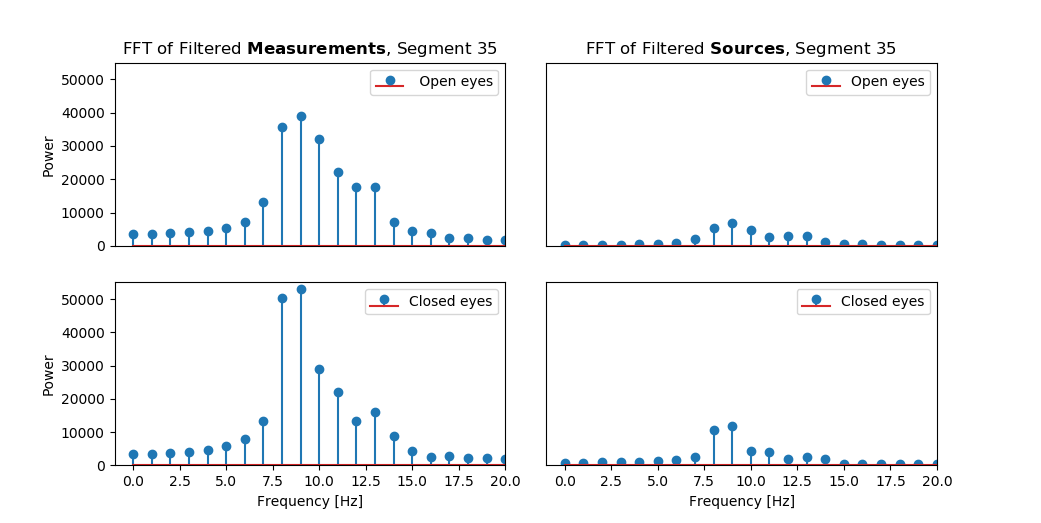
\includegraphics[scale=0.5]{figures/ch_7/FFT_plot.png}
\caption{power spectrum of the filtered EEG measurements and source signals of time segment 35 for open and closed eyes data set of test subject 1.}
\label{fig:dft_2}
\end{figure}
\noindent
By observing figure \ref{fig:dft_2} it is seen, for the specific segment, that the power within the alpha band is significantly larger within the EEG measurements compared to the sources. 
Furthermore, is it seen for both the EEG measurements and the source signals that the power has increased from open to closed eyes. 
Considering the calculated relations is it seen the that biggest increase in power is found on source level. 
This behavior does support the theory, however the result of a single segment is not sufficient to draw any conclusion.          

Figure \ref{fig:dft_5} and \ref{fig:dft_6} illustrate the $C/O$ relation computed for the 100 time segments, of the EEG measurements and source signals respectively. 
The horizontal line in the plots marks the 1/1 relation.
As such the segments where the highest power was found for closed eyes lies above the line - supporting the theory. Opposite the segments with least power found for closed eyes lies below the line.      
\begin{figure}[H]
\begin{widepage}
    \begin{minipage}[t]{.49\textwidth}
\centering
\includegraphics[width=1\linewidth]{figures/ch_7/DFT_Y_Difference.png}
\caption{The $C/O$ relation for EEG measurements for 100 time segments. The average $C/O$ over all segments is $1.16$.}
\label{fig:dft_5}
\end{minipage} 
\hspace{.5cm}
\begin{minipage}[t]{.49\textwidth}
\centering
\includegraphics[width=1\linewidth]{figures/ch_7/DFT_X_Difference.png}
\caption{The $C/O$ relation of source signals for 100 time segments. The average $C/O$ over all segments is $2.01$.}
	\label{fig:dft_6}
    \end{minipage}
\end{widepage}
\end{figure}
\noindent
From the figures it is clear the behavior seen from the example of segment 35, is not a continuous behavior. 
It is seen both on EEG level and source level that relation scatters around the horizontal line, indicating that the relation is not stationary over time.  
On figure \ref{fig:dft_6} is it seen that the $C/O$ relation range from near zero to beyond 20 for a few segments, indicating a significant change in power compared to figure \ref{fig:dft_5}. 
With 57 out of 100 segments lying below the horizontal line the behavior is considered more or less random. 
From these observations the expected behavior was not found. 
This does support the earlier findings with respect to the main algorithm, indicting a significant unreliability to the result. 

With respect to the method for computing the $C/O$ relation it could be considered whether computing the relation for every segment is the right choice. 
One could argue that summing the power over all segments for respectively open and closed eyes and then compute the $C/O$ relation would yield a different result.  